% The chord and the retrospective look-behind sweep.
% TryAllNavigator.hpp:340-346
%   step          = stepEnd - stepStart          (the chord)
%   stepDirection = step.normalized()            (chord direction, not tangent)
%   nearLimit     = -stepDistance + tolerance
%   farLimit      = 0
%   resolveTargets(state, stepEnd, stepDirection, nearLimit, farLimit)
\documentclass[border=8pt]{standalone}
\usepackage{tikz}
\usepackage{newtxtext,newtxmath}
\usetikzlibrary{arrows.meta,positioning,calc,decorations.pathreplacing}

\begin{document}
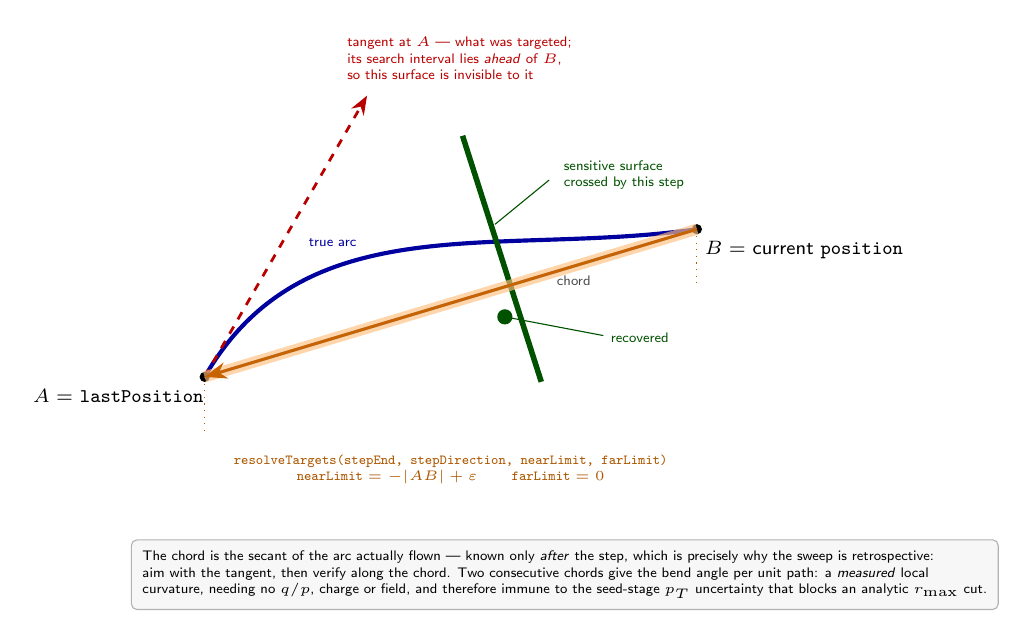
\begin{tikzpicture}[
  scale=1.25,
  font=\sffamily\footnotesize,
  arc/.style={line width=1.5pt,draw=blue!62!black},
  tang/.style={line width=1.0pt,draw=red!72!black,dashed,-{Stealth[length=2.4mm]}},
  chord/.style={line width=1.1pt,draw=black!75},
  surf/.style={line width=2.0pt,draw=green!32!black},
  pt/.style={circle,fill=black,inner sep=1.3pt},
  lbl/.style={font=\sffamily\scriptsize},
  tny/.style={font=\sffamily\tiny}
]

% ---- the step actually flown ----
\draw[arc] (0,0) to[out=60,in=188] (5.0,1.50);
\coordinate (A) at (0,0);
\coordinate (B) at (5.0,1.50);

% ---- the missed surface ----
\draw[surf] (3.42,-0.05) -- (2.62,2.45);
\node[tny,text=green!32!black,anchor=west,align=left] at (3.55,2.05)
  {sensitive surface\\ crossed by this step};
\draw[draw=green!32!black,line width=0.4pt] (3.50,2.00) -- (2.95,1.55);

% ---- tangent at A ----
\draw[tang] (A) -- ++(60:3.3);
\node[tny,text=red!72!black,anchor=south west,align=left] at (1.35,2.92)
  {tangent at $A$ --- what was targeted;\\ its search interval lies \emph{ahead} of $B$,\\
   so this surface is invisible to it};

% ---- the chord ----
\draw[chord] (A) -- (B);
\node[pt] at (A) {}; \node[pt] at (B) {};
\node[lbl,anchor=north east,inner sep=2pt] at (0.05,-0.06) {$A=$ \texttt{lastPosition}};
\node[lbl,anchor=north west,inner sep=2pt] at (5.02,1.44) {$B=$ current \texttt{position}};
\node[tny,text=black!70,anchor=north,inner sep=2.5pt] at (3.75,1.10) {chord};
\node[tny,text=blue!62!black,anchor=south,inner sep=1.5pt] at (1.30,1.28) {true arc};

% ---- the look-behind search interval, offset below the chord ----
\begin{scope}[shift={(0,-0.55)}]
  \draw[line width=4.0pt,draw=orange!50,opacity=0.65] (A) -- (B);
  \draw[-{Stealth[length=2.8mm]},line width=1.0pt,draw=orange!78!black] (B) -- (A);
  \node[tny,text=orange!68!black,anchor=north,align=center] at (2.5,-0.14)
    {\texttt{resolveTargets(stepEnd, stepDirection, nearLimit, farLimit)}\\
     \texttt{nearLimit} $=-|AB|+\varepsilon$ \qquad \texttt{farLimit} $=0$};
\end{scope}
\draw[draw=orange!70!black,line width=0.4pt,dotted] (A) -- ($(A)+(0,-0.55)$);
\draw[draw=orange!70!black,line width=0.4pt,dotted] (B) -- ($(B)+(0,-0.55)$);

% ---- the recovered hit ----
\fill[green!32!black] (3.05,0.61) circle (2.2pt);
\draw[draw=green!32!black,line width=0.4pt] (3.05,0.61) -- (4.05,0.42);
\node[tny,text=green!32!black,anchor=west,inner sep=1.5pt] at (4.08,0.40) {recovered};

% ---- caption ----
\node[draw=black!30,fill=black!3,rounded corners=2pt,inner sep=4pt,
      align=left,tny,anchor=north west] at (-0.75,-1.65)
  {The chord is the secant of the arc actually flown --- known only \emph{after} the step, which is
   precisely why the sweep is retrospective:\\
   aim with the tangent, then verify along the chord. Two consecutive chords give the bend angle per
   unit path: a \emph{measured} local\\
   curvature, needing no $q/p$, charge or field, and therefore immune to the seed-stage $p_T$
   uncertainty that blocks an analytic $r_{\max}$ cut.};

\end{tikzpicture}
\end{document}
